The desired outcome of this thesis will be a working Android app prototype with working CRUD functions for knitting chart patterns and a row counter functionality while viewing a pattern. This prototype is intended as an aid for knitters of all backgrounds during their respective knitting projects. Patterns will be saved locally as a \gls{json} file on the device's internal storage. It would also be an option to store patterns on a server and let the app play the role of client, but that would not fit within the time constraints of this thesis. To give the user the ability to backup their patterns the app will support the import and export of pattern from external storage. For a detailed explanation of Android's concepts of internal and external storage see section \ref{storage}. Patterns exported will be accessible by the user and can be handled in whatever way the user sees fit to, for example, share or upload a pattern.

A chart pattern will consist of a set number of rows and columns. Each cell of the grid contains a symbol representing a knitting stitch. Created pattern are stored locally on the device and can be manipulated by the user in-app, as CRUD operations apply. Creating, editing and viewing patterns will be based on two shared visual formats for the pattern: a grid format and a row format.

The grid format will display the pattern in a grid, simulating the most common form of commercial distribution for knitting chart patterns on both analogue and digital media. Manipulation of the pattern content will be possible through a software keyboard containing the stitch symbols. A symbol can be selected and then applied to cells in the grid via touch. The symbol will stay active until the user selects a different symbol. The grid size can be changed with a button which opens a dialog where the desired amount of rows and columns can be entered. On confirmation the grid will shrink or expand to the set dimensions. Any symbols lying outside of the new bounds will be deleted, whereas new cells will be empty.

Similar to the grid format the row format will display the pattern rows, but will forego the representation of the columns. Instead the cells of a row will be summarized in such a way, that consecutive, identical symbols will be represented  by a number value equal to the count of the symbols and followed by the stitch symbol. Rows in this format can be edited like a conventional text editor - a movable cursor to show where further user input will be inserted and text selection functions for multiple character deletion, copying and pasting will be available. The software keyboard corresponding to this format will consist of the stitch symbols and a num pad, as well as an enter and a backspace key.

Viewing a pattern will come with a row counter below the actual chart pattern. This counter can be increased, decreased and reset by utilizing buttons. The counter is limited between one, as the first row of a pattern, and the number of rows the pattern contains in total. The current row will be indicated through a highlight on the pattern, marking the corresponding row in both grid and row format. When exiting the viewer the current row number will be saved in the pattern file and applied to the counter the next time the pattern is viewed

While editing or viewing a pattern, the row and the grid format will allow the user to 2D scroll, meaning both vertical and horizontal scroll. Additionally, the grid view can be zoomed and reset to default zoom and scroll. Switching between both formats while editing and viewing a pattern will be supported with a button. Upon switching the pattern will be saved. Renaming, deleting, saving, and exporting the pattern will be possible from within both formats with menu entries.

On app launch the list of patterns saved on the device will be shown. While viewing that list menu entries for exporting all patterns and importing a single pattern will be available. For the import the user can choose a file on the device from a file chooser. Exporting will export files to a set directory on the publicly accessible storage of the device. A list item will consist of the pattern name, an edit, and a delete button. A click on the pattern name will open the pattern in the viewer in row format with the default dimensions of 10 columns and 10 rows. Below the list will be a button to create a new pattern which will open a dialog for entering the new pattern’s name. After confirming a name, the editor will open with the row format.

\begin{figure}
  \centering
  \begin{minipage}{1\textwidth}
    \centering
    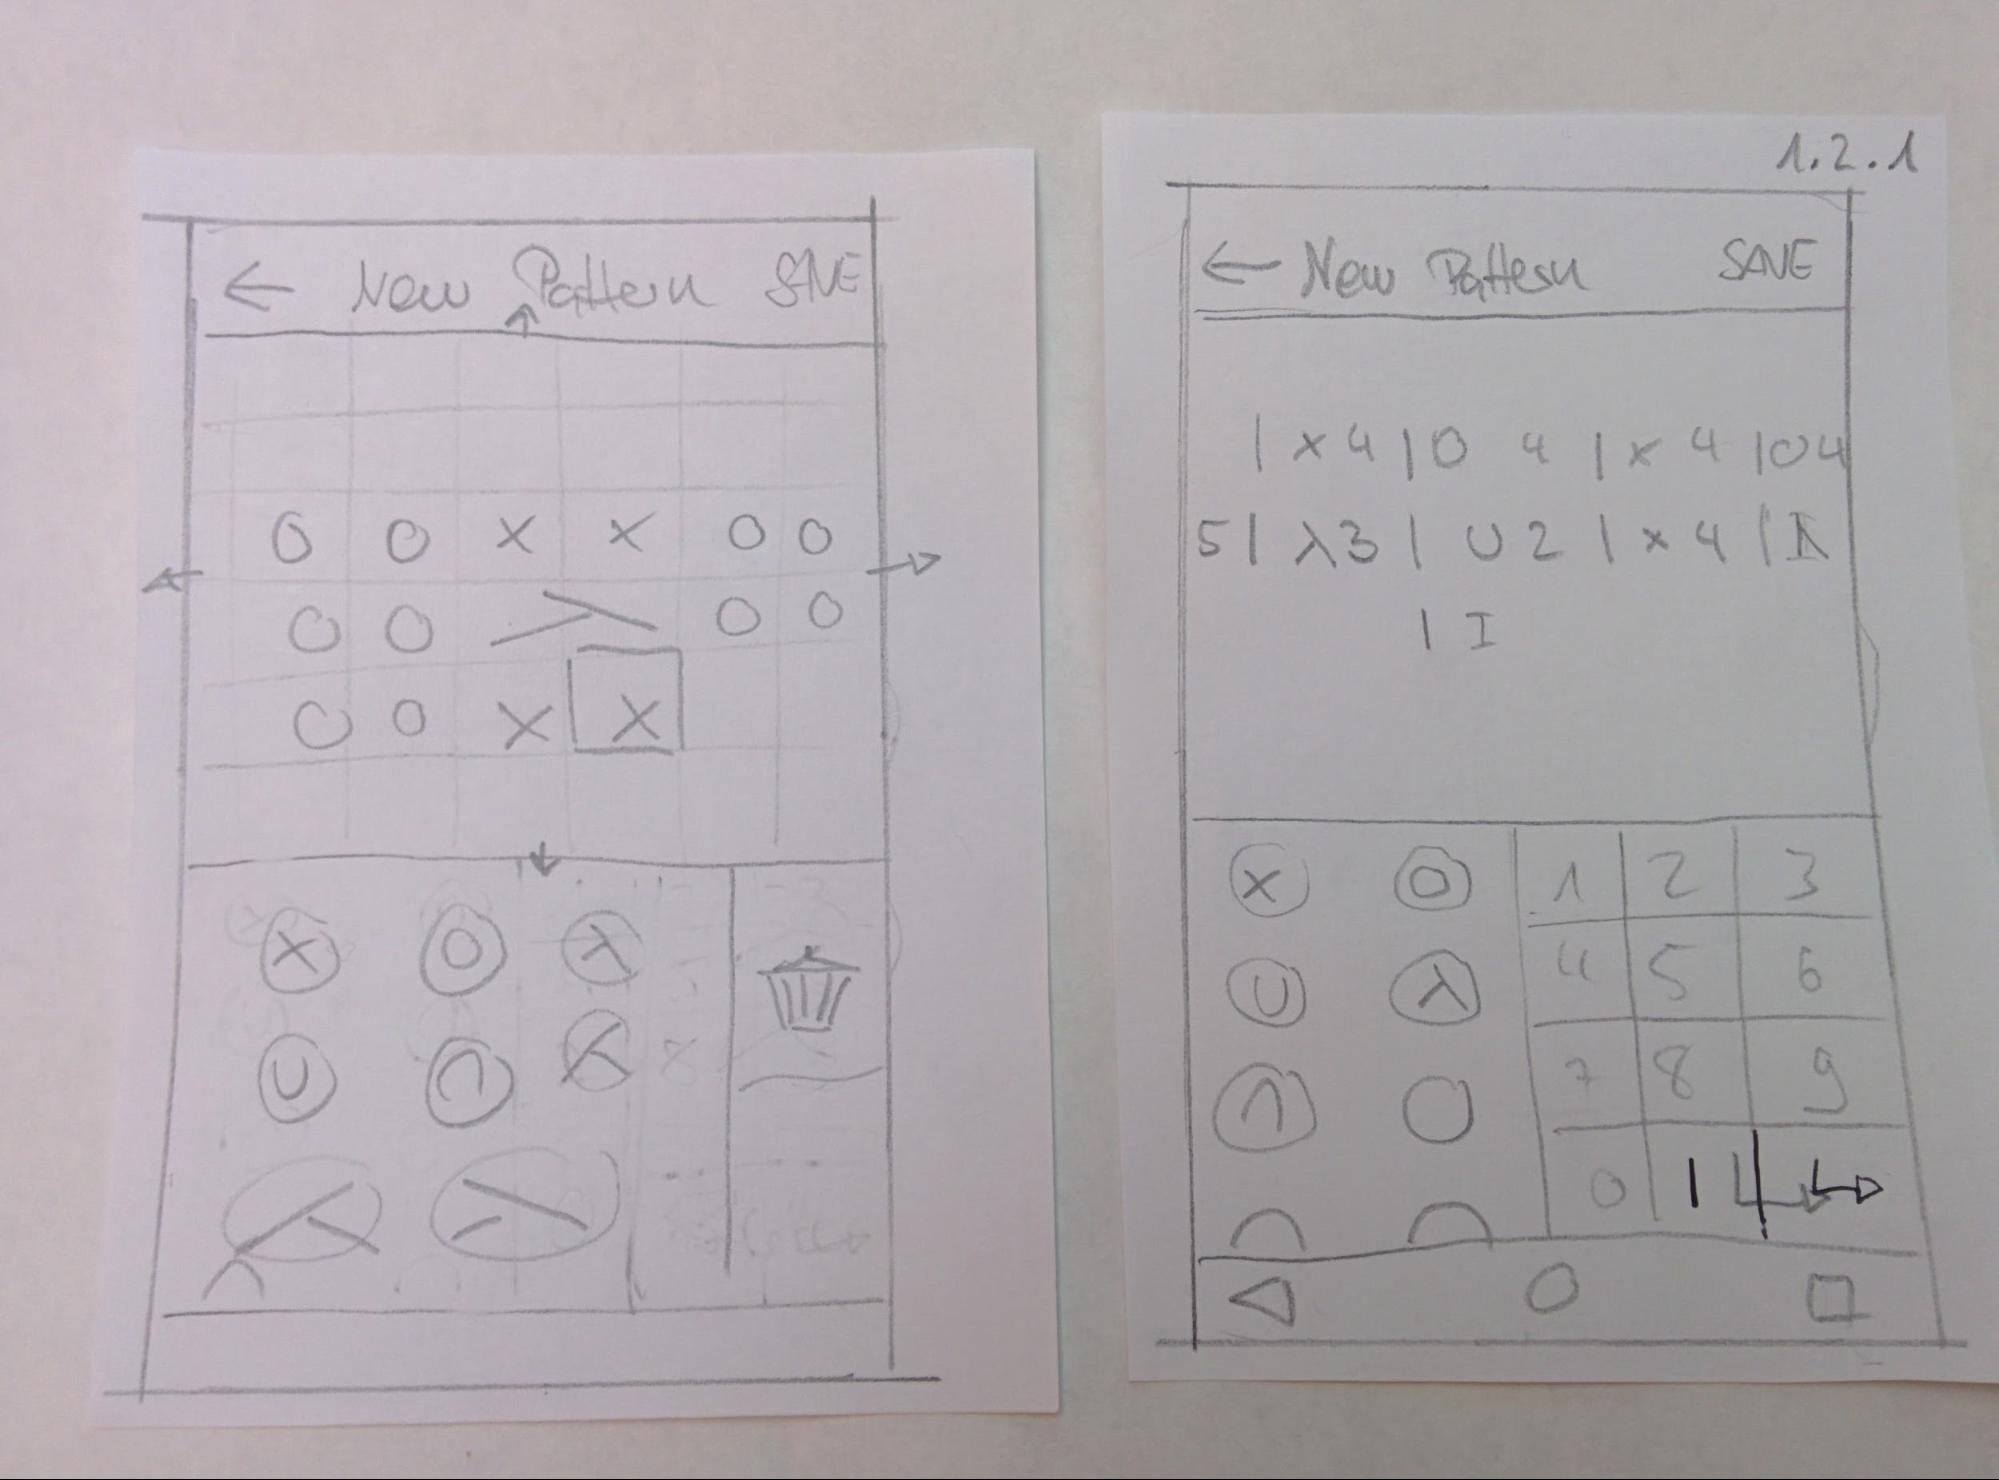
\includegraphics[width=1\linewidth]{images/image09.jpg}
    \caption{Editor screens for grid and row format with pattern name and save button in navigation bar}
    \label{fig_wireframe1}
  \end{minipage}

  \begin{minipage}{1\textwidth}
    \centering
    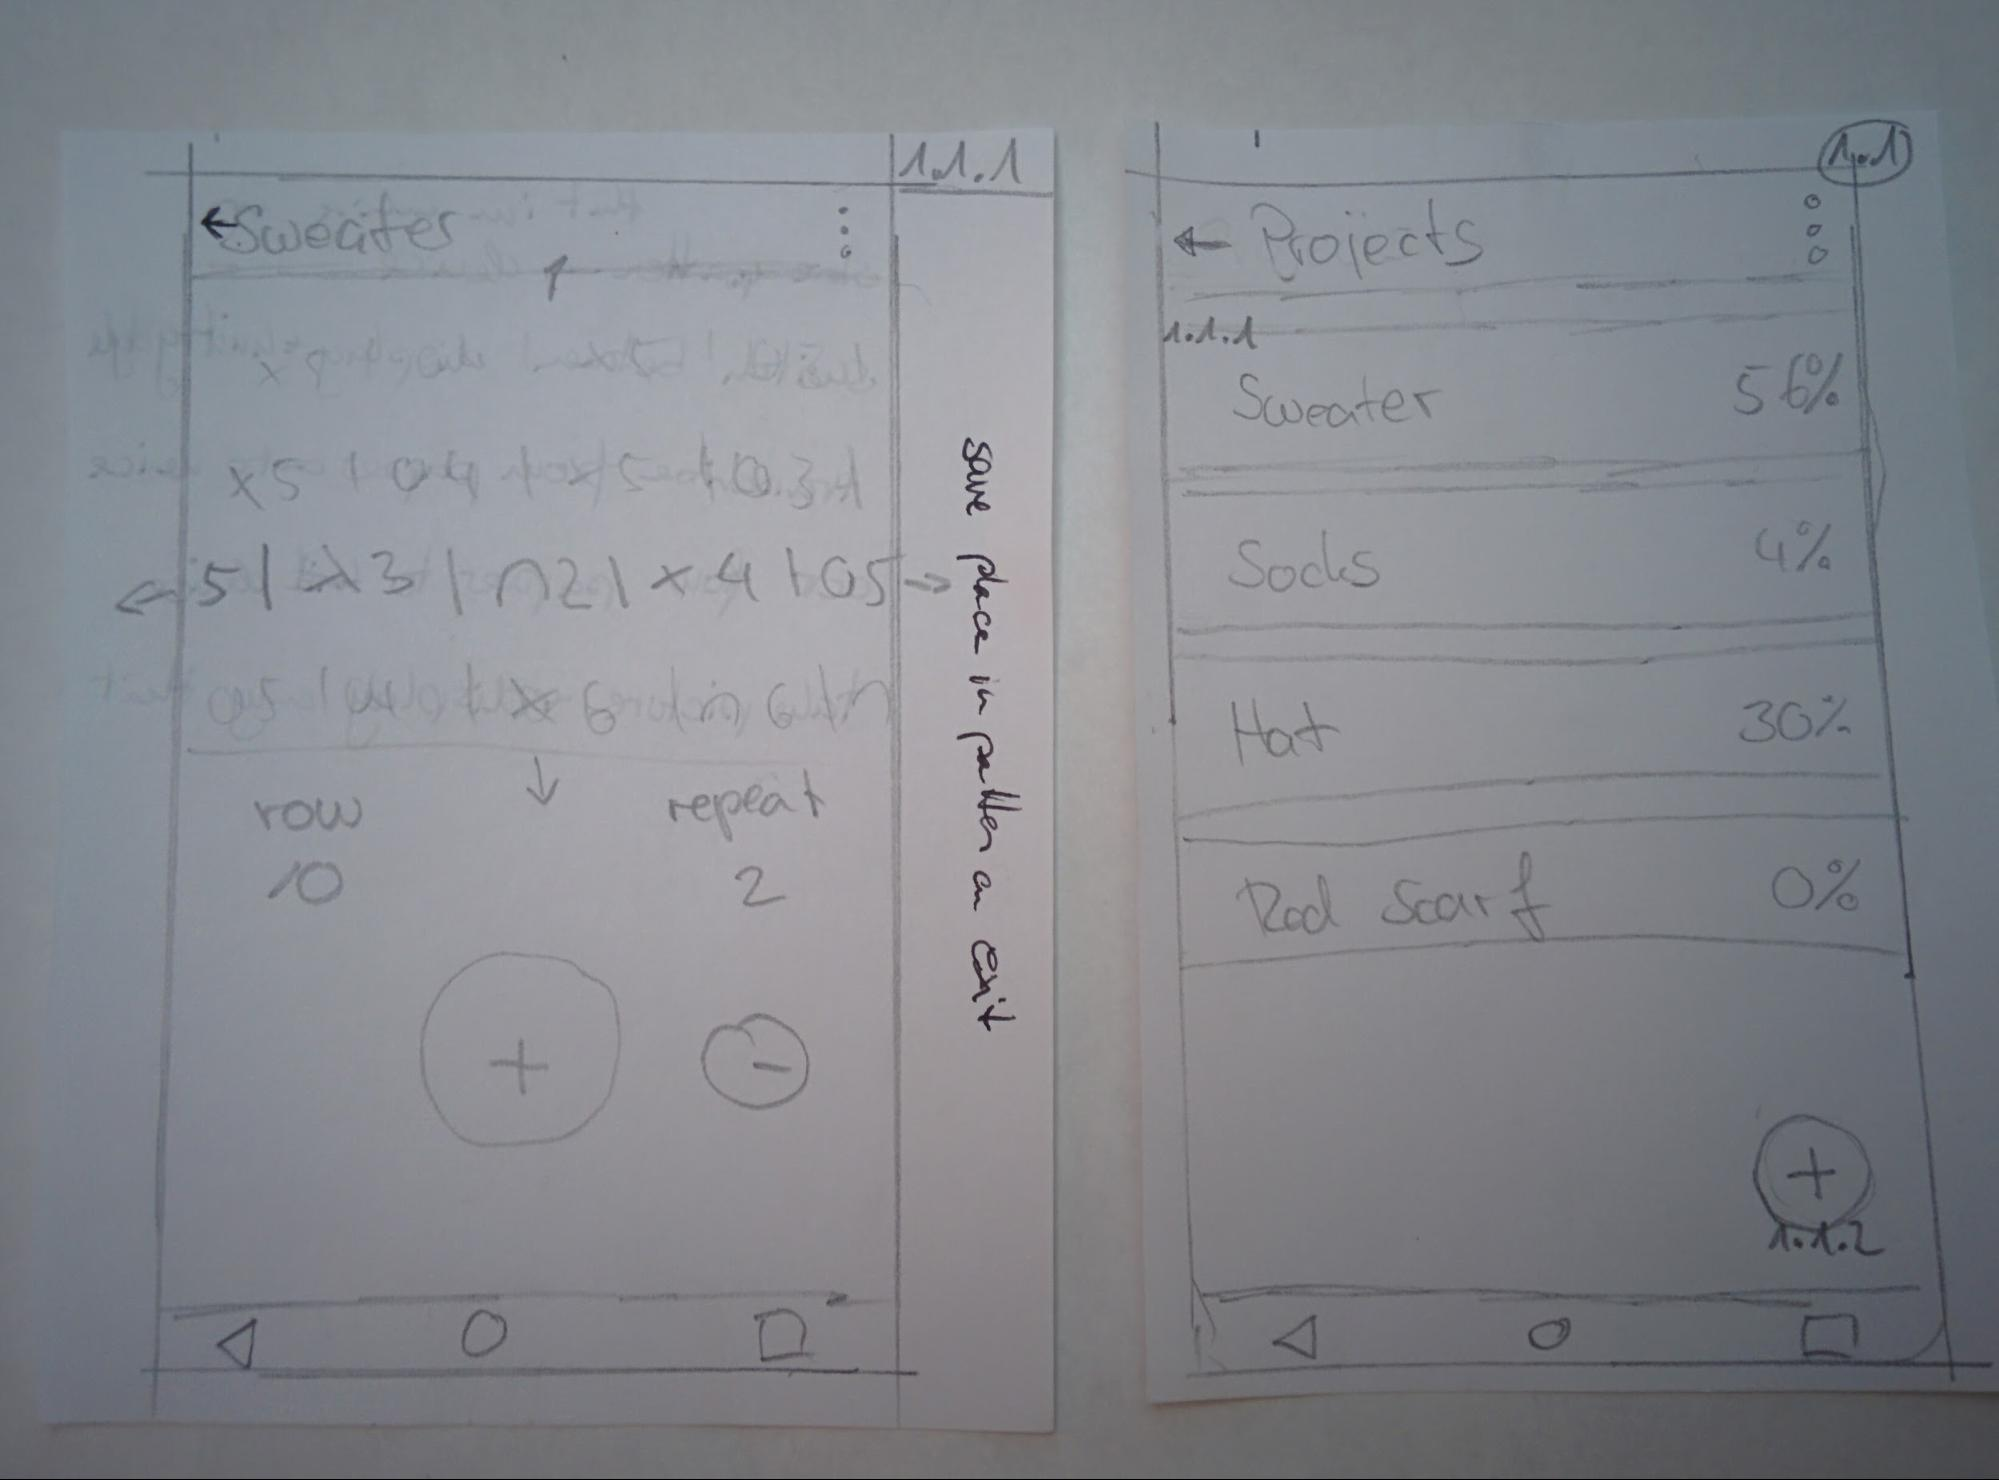
\includegraphics[width=1\linewidth]{images/image08.jpg}
    \caption{Viewer screen for row format and selection screen for stored patterns}
    \label{fig_wireframe2}
  \end{minipage}

  \caption{Screens for editor and viewer without Android elements}
\end{figure}

\begin{figure}
\centering
\begin{minipage}{1\textwidth}
  \centering
  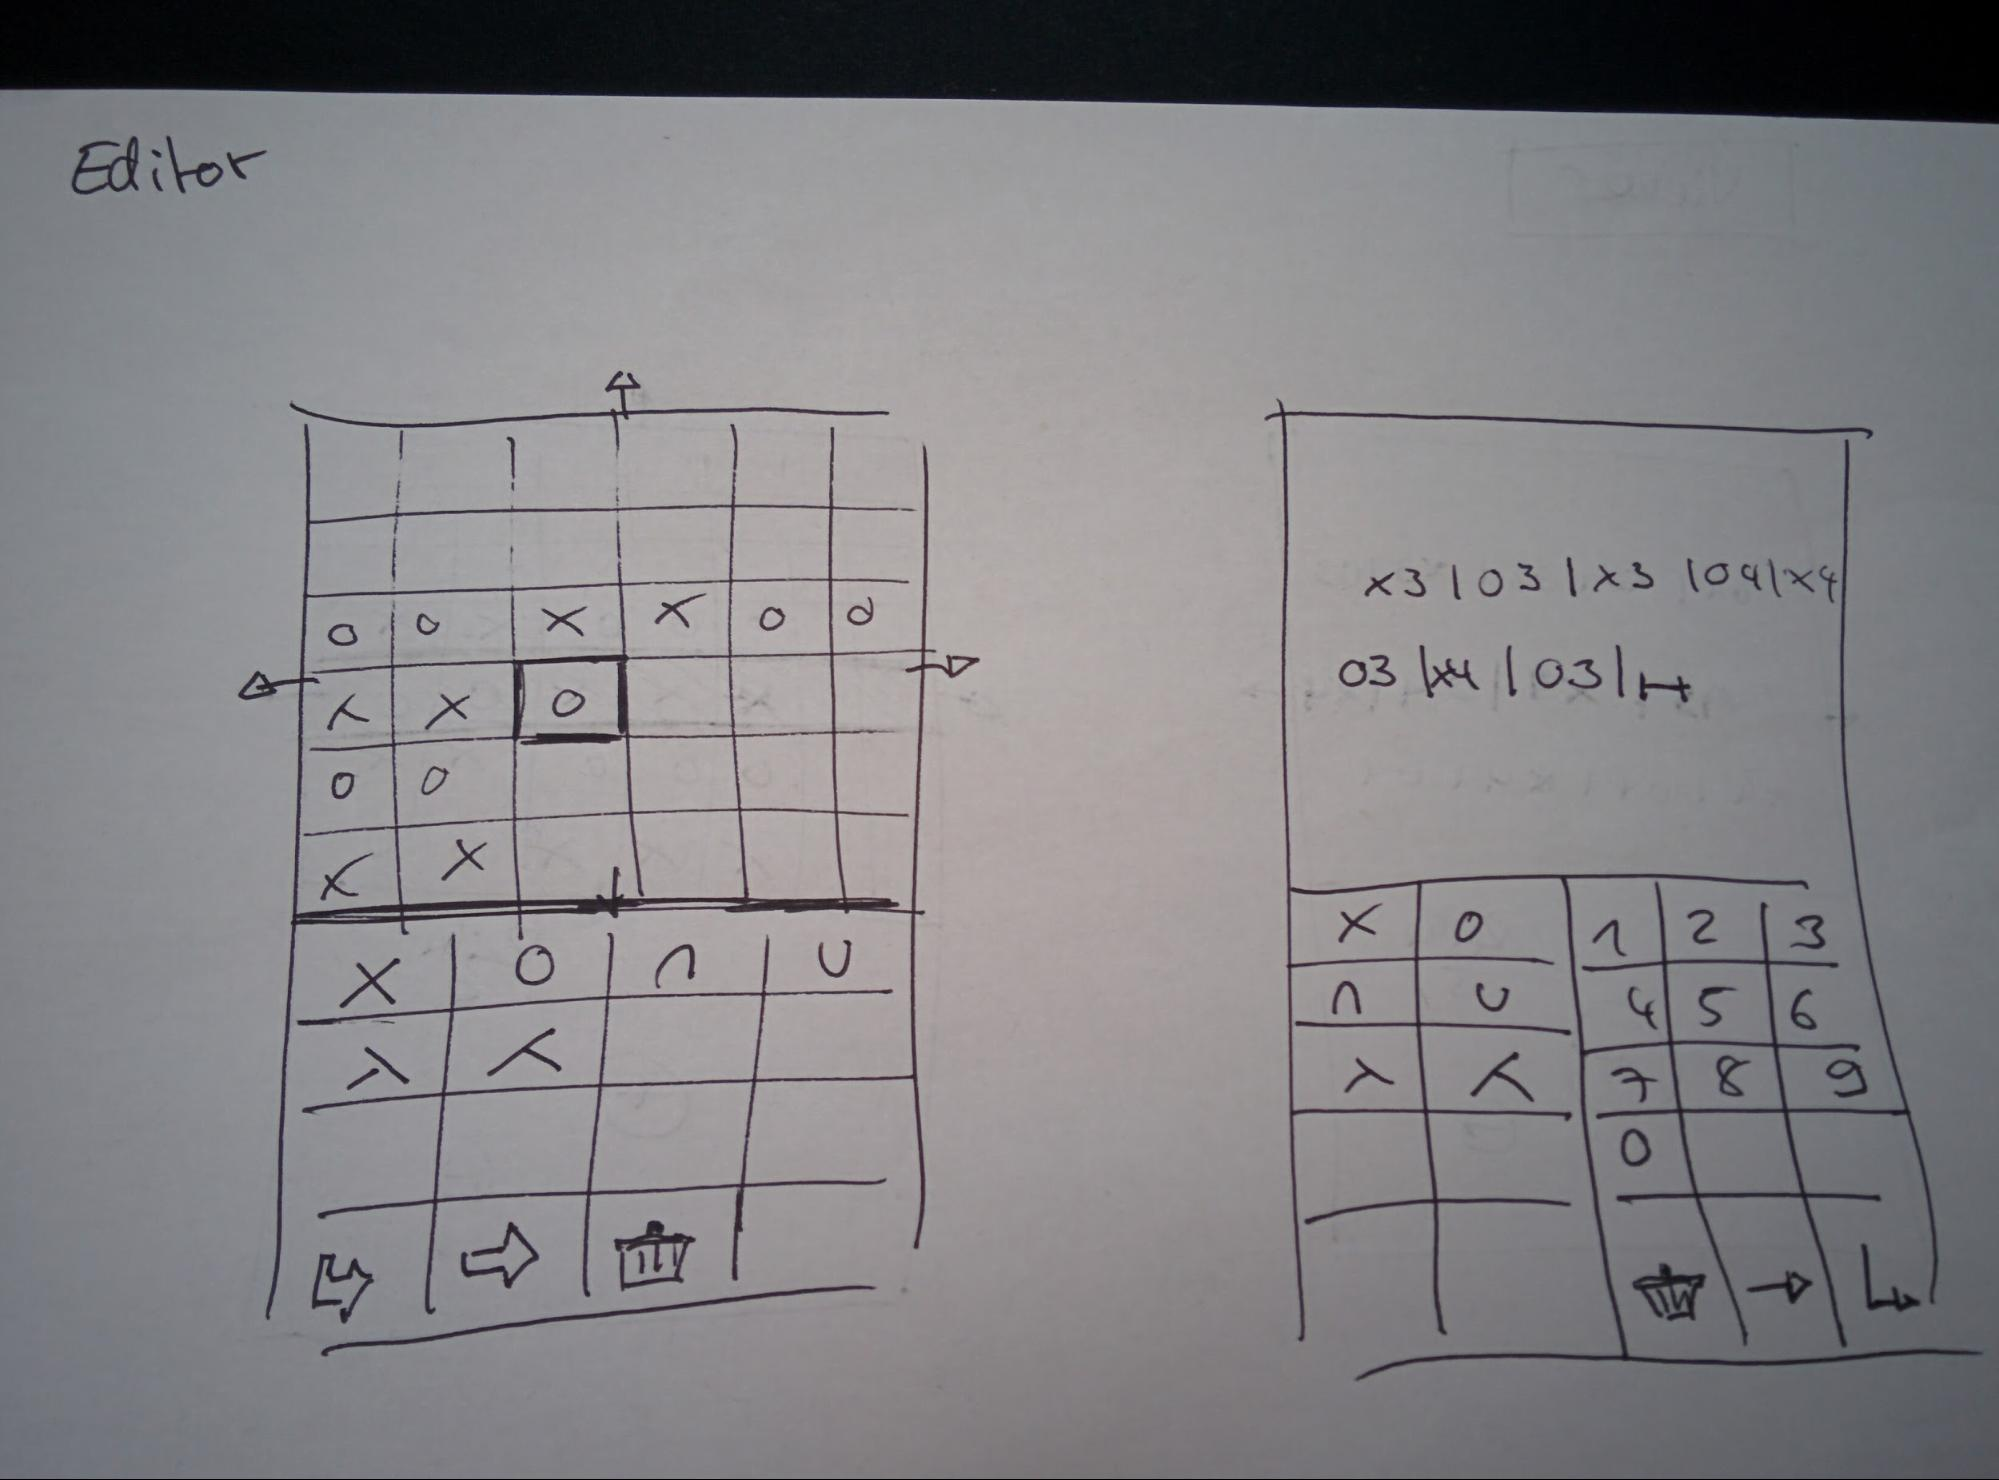
\includegraphics[width=1\linewidth]{images/image00.jpg}
  \caption{Editor screens for grid and row format}
  \label{fig_wireframe3}
\end{minipage}

\begin{minipage}{1\textwidth}
  \centering
  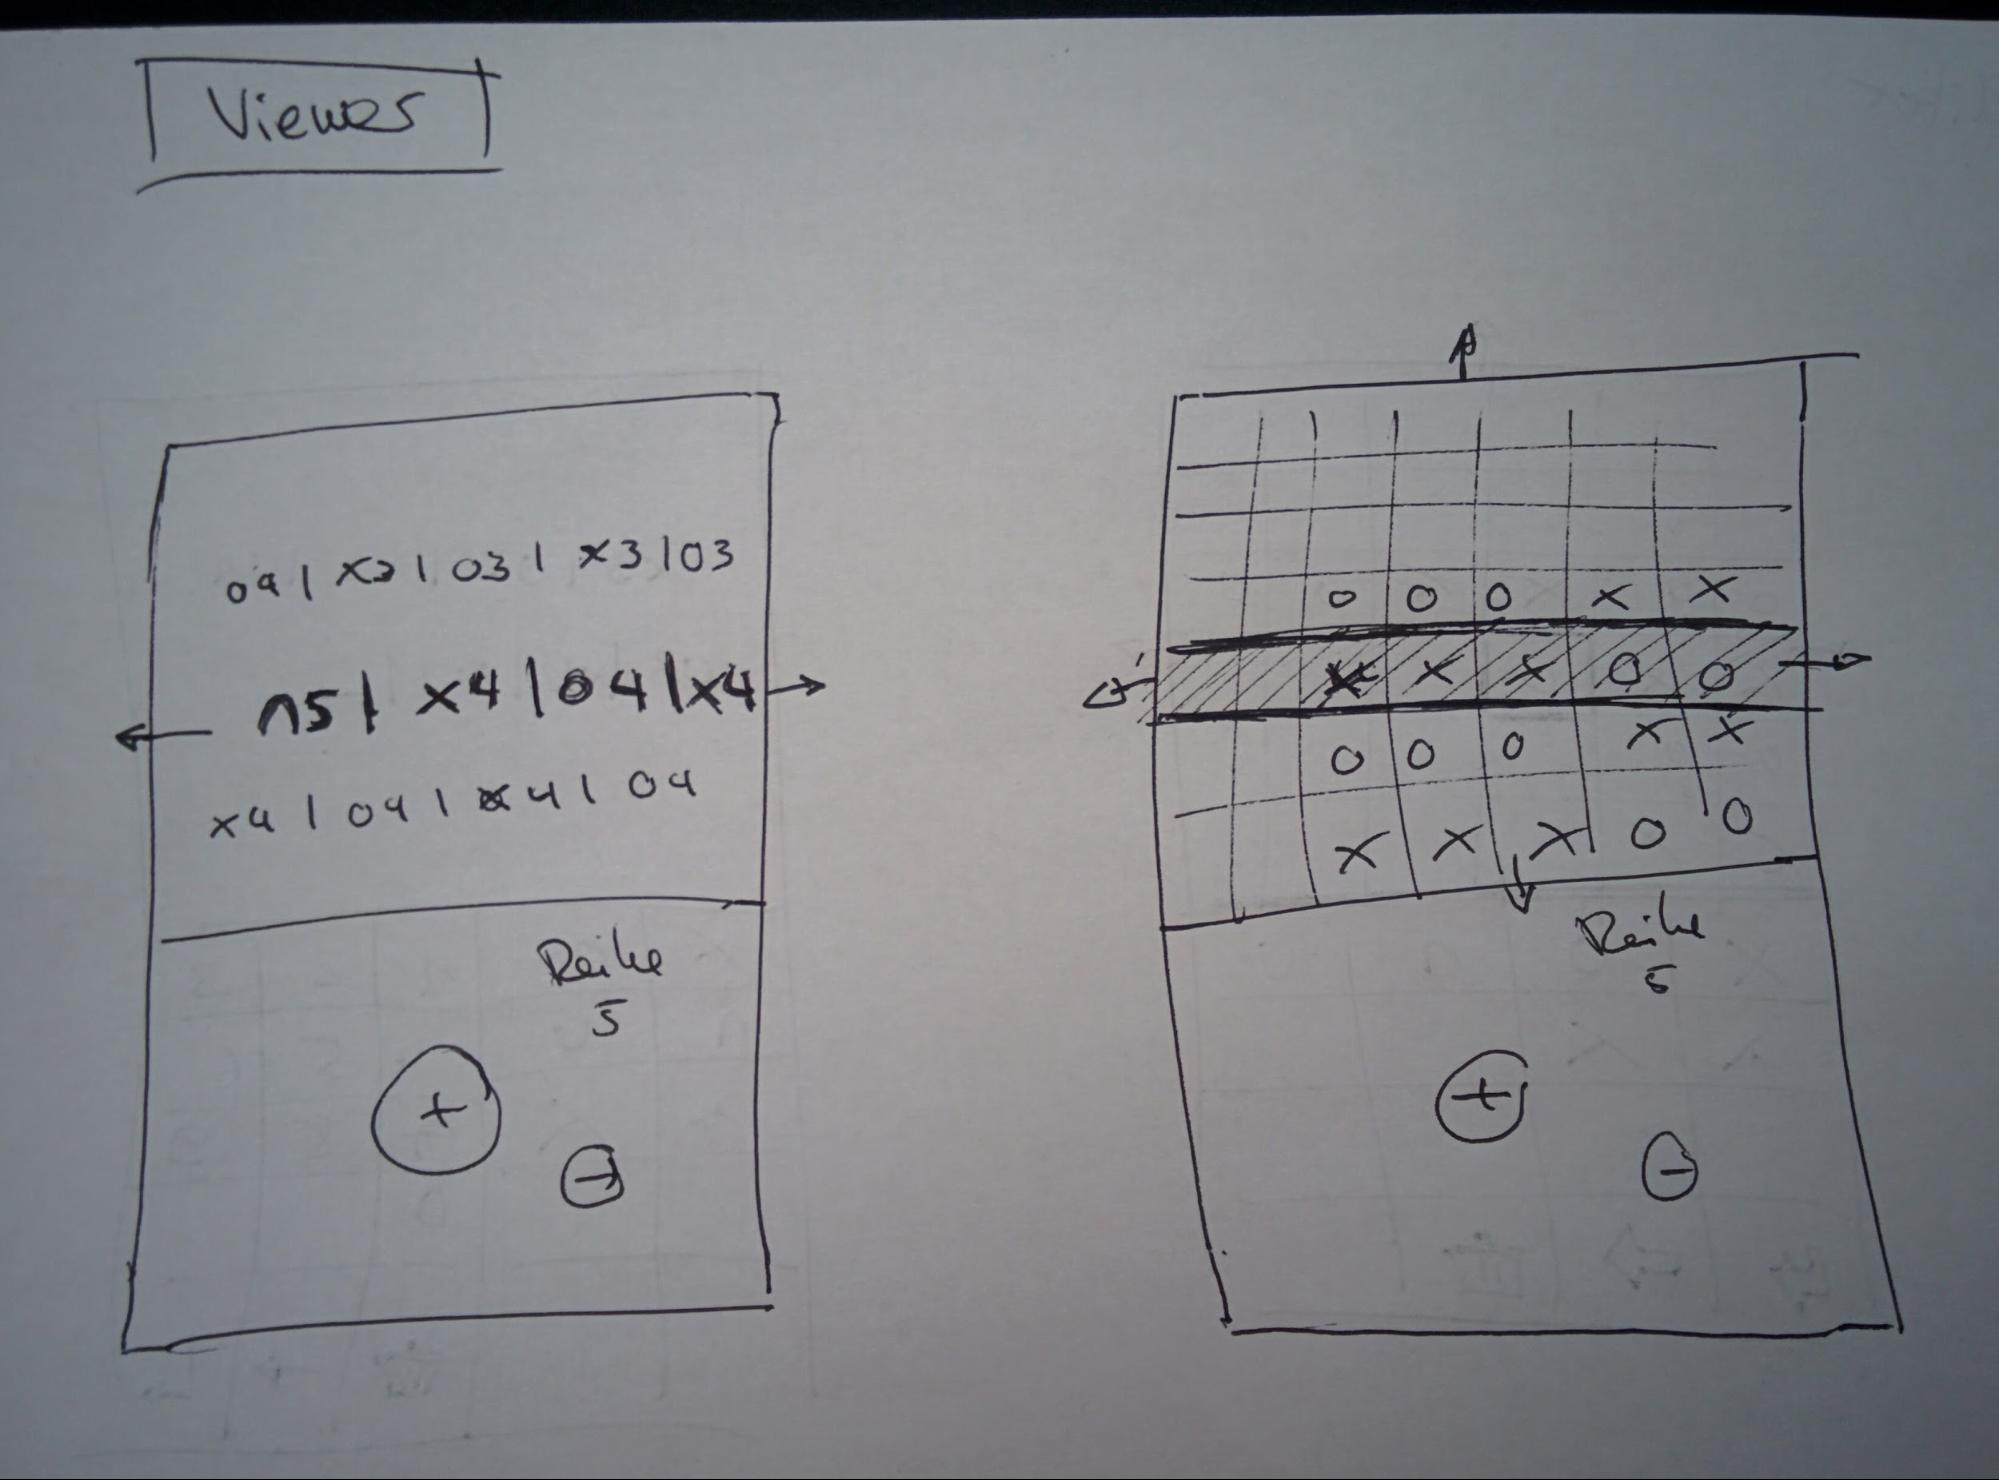
\includegraphics[width=1\linewidth]{images/image02.jpg}
  \caption{Viewer screens for grid and editor format with row counter}
  \label{fig_wireframe4}
\end{minipage}
\end{figure}